\documentclass[border=6pt]{standalone}
\usepackage{tikz}
\usepackage[edges]{forest}
\usetikzlibrary{arrows.meta,positioning,calc,decorations.pathreplacing,shapes.geometric}
\begin{document}
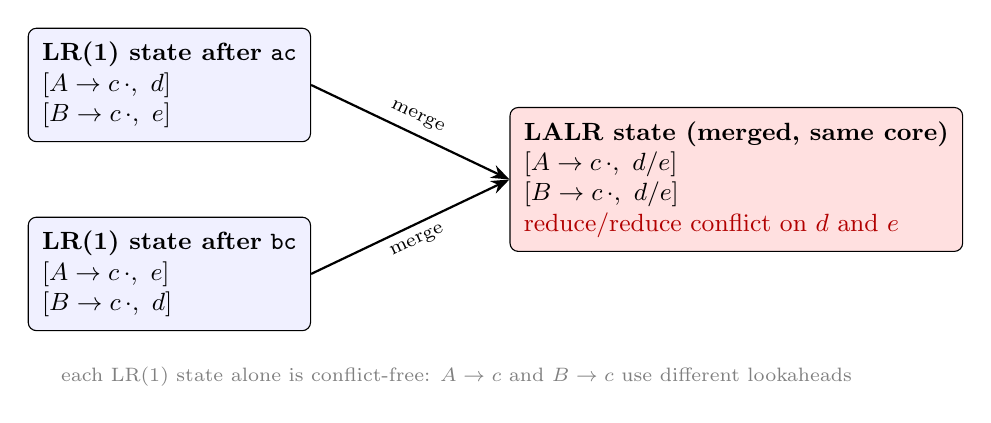
\begin{tikzpicture}[>=Stealth,font=\small,
 st/.style={draw,rounded corners=3pt,align=left,inner sep=5pt,fill=blue!6}]
\node[st] (a) at (0,1.2) {\textbf{LR(1) state after} \texttt{ac}\\ $[A \to c\,\cdot,\ d]$\\ $[B \to c\,\cdot,\ e]$};
\node[st] (b) at (0,-1.2) {\textbf{LR(1) state after} \texttt{bc}\\ $[A \to c\,\cdot,\ e]$\\ $[B \to c\,\cdot,\ d]$};
\node[st,fill=red!12] (m) at (7.2,0) {\textbf{LALR state (merged, same core)}\\ $[A \to c\,\cdot,\ d/e]$\\ $[B \to c\,\cdot,\ d/e]$\\ \textcolor{red!70!black}{reduce/reduce conflict on $d$ and $e$}};
\draw[->,thick] (a.east) -- node[above,sloped,font=\scriptsize]{merge} (m.west);
\draw[->,thick] (b.east) -- node[below,sloped,font=\scriptsize]{merge} (m.west);
\node[font=\scriptsize,gray,anchor=west] at (-1.5,-2.5) {each LR(1) state alone is conflict-free: $A \to c$ and $B \to c$ use different lookaheads};
\end{tikzpicture}
\end{document}
